\documentclass[11pt]{article}
\usepackage[margin=1in]{geometry}
\usepackage{amsmath,amssymb,booktabs,graphicx,microtype}
\usepackage[T1]{fontenc}
\usepackage{lmodern}
\usepackage[hidelinks]{hyperref}
\usepackage{enumitem}
\usepackage{natbib}
\setlist{nosep,leftmargin=1.5em}
\graphicspath{{../figures/}}

\title{\bfseries Finding the minimal attention circuit during training\\
       with hemodynamic attenuation}
\author{Anonymous authors\\ \small Paper under double-blind review}
\date{}

\begin{document}
\maketitle

\begin{abstract}
\noindent
A trained transformer usually has many more attention heads than its task needs. We ask
whether training can find the smallest set of heads by itself, without being told how many
to keep. We give each head a valve and, during training, close a head when the other heads
can take over its job, the way a blood vessel can be pruned when collateral vessels supply
its tissue, and fade it out gradually, the way unused vessels regress. We call this
\emph{hemodynamic attenuation}. The value we use for each head, the loss that remains after the other heads
re-fit to cover for it, is a classical pruning score (Optimal Brain Surgeon, ZipLM). What is
new is how it is used: from the start of training, with a price per head instead of a target
size, and with heads fading out gradually. We test this on a retrieval task whose minimal
number of heads $k^\star$ is known from a simple counting argument. Across $k^\star = 2$ to $8$,
the rule kept exactly $k^\star$ heads in 47 of 50 runs and never broke the trained model (50 of 50).
Every other rule we tested got at most one of the two: ordinary importance kept the wrong number,
random choice and standard pruning broke the model, and learned gates got neither reliably. Using the same
score the usual way, all at once after training, also found the count but broke the model in
every run (30 of 30). When heads can fail at random, a formula written before the experiments
predicted how many backup heads the rule keeps (21 of 24 runs exactly, the rest off by one).
\end{abstract}

\section{Introduction}

Circuit analysis is easier when a model has few components. Most methods find a small circuit
\emph{after} training: they rank heads in a trained model and remove the low-ranked ones until a
chosen size or speed is reached \citep{michel,voita,ziplm,kwon}. Two things are then fixed by
hand: how many heads to keep, and the moment to cut. We ask instead whether training itself can
discover the minimal set, and we test the answer on a task where the right number is known.

The rule borrows one idea from blood flow in the brain. When a vessel is lost, tissue survives if
neighbouring (collateral) vessels can supply it, and vessels that carry little flow are pruned
gradually rather than cut. So the question asked of each head is not ``how much does it carry?''
but ``what would nobody else carry if it were gone?''. The same idea has a long history in
pruning as a second-order or re-fitted score \citep{obd,obs,ziplm,kwon}; we do not claim the
score. Our contributions are:
\begin{enumerate}
\item A retrieval task whose minimal head count is fixed by the task itself, with the exact best
      loss for any smaller number of heads, confirmed by experiment (Section~\ref{sec:task}).
\item A rule that uses the re-fitted score \emph{during} training, with a price instead of a
      target and gradual fading, and finds the minimal count without leaving the solved region
      (Sections~\ref{sec:rule}--\ref{sec:results}).
\item A prediction, made before the runs, of how many backup heads the rule keeps when heads can
      fail (Section~\ref{sec:backup}).
\end{enumerate}

\begin{figure}[t]
\centering
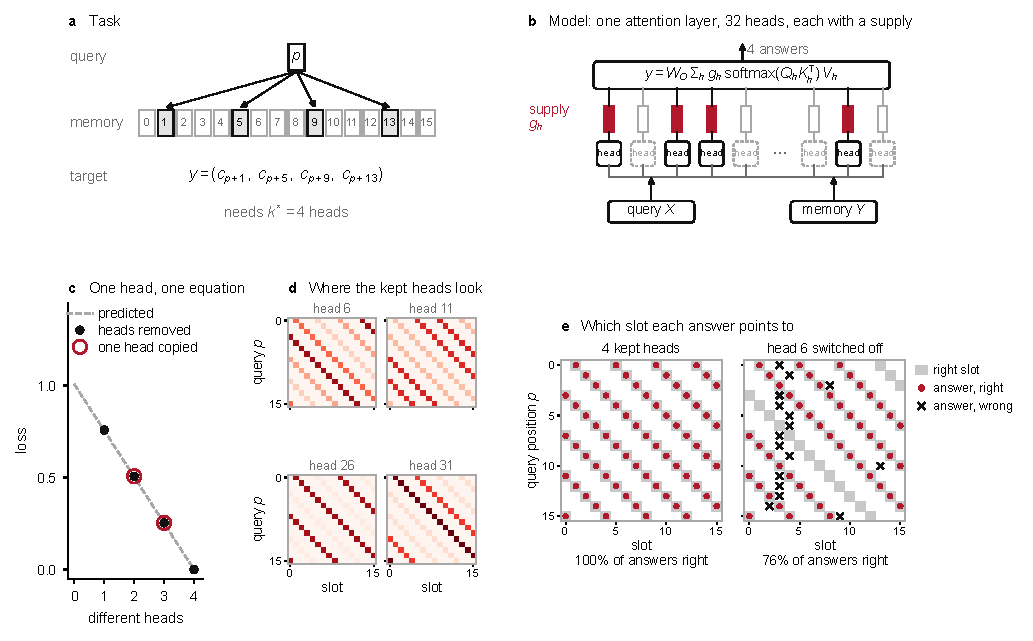
\includegraphics[width=\linewidth]{fig_setup.pdf}
\caption{\textbf{Task, model, and what ``solved'' looks like.}
\textbf{a}, A query carries a position $p$; the answer is the four items stored $1, 5, 9, 13$
slots ahead (wrapping round), so 4 heads are needed.
\textbf{b}, One attention layer with 32 heads; each head's output passes through a valve $g_h$
before the output weights. Filled valves are open.
\textbf{c}, Best loss with $k$ different heads on, measured on a trained 4-head model with the other heads
switched off (dots) or with all 4 on but some replaced by copies of another (circles), against the prediction
$1 - k/4$: a copy adds nothing, each different head adds one answer.
\textbf{d}, Which memory slot each of the model's answers points to (the nearest stored item).
Grey squares are the right slots. With the 4 kept heads, every answer is right (100\% of 65{,}536
held-out answers). With head 6 switched off, the answers for $p + 13$ become wrong (crosses),
76\% right overall.}
\label{fig:setup}
\end{figure}

\section{The task}
\label{sec:task}

\paragraph{In words.} There is a memory of $N$ numbered slots, and each slot holds a random item.
A query names a position $p$. The model must return the items found at $R$ fixed distances
$\delta_1, \dots, \delta_R$ ahead of $p$, counting round the memory like a clock:
\begin{equation}
\text{answer}(p) = \big(c_{p+\delta_1},\ c_{p+\delta_2},\ \dots,\ c_{p+\delta_R}\big),
\qquad \text{slot numbers taken mod } N,
\label{eq:task}
\end{equation}
where $c_j$ is the item in slot $j$. The items are drawn fresh for every example, so they cannot
be memorised; the model has to learn \emph{where to look}.

\paragraph{A tiny example.} Take $N = 8$ slots and $R = 2$ distances, $\delta = (1, 5)$. A query
with $p = 6$ needs slots $(6 + 1) \bmod 8 = 7$ and $(6 + 5) \bmod 8 = 3$, so the answer is
$(c_7, c_3)$. A query with $p = 2$ needs slots 3 and 7, so the answer is $(c_3, c_7)$. Wrapping
round (``mod $N$'') means every position has all $R$ answers inside the memory, and ``look 5
ahead'' is the same rule at every position.

\paragraph{As matrices.} Each example has $N$ memory rows and $N$ query rows; every row is a vector
of length $d$. Memory row $j$ is the slot's label next to its item; query row $i$ is the label of
the position it asks about:
\[
Y_j = \big[\, e_j \;\big|\; c_j \;\big|\; \text{noise} \,\big], \qquad
X_i = \big[\, e_{p_i} \;\big|\; \text{noise} \,\big], \qquad
T_i = \big[\, c_{p_i+\delta_1} \;\big|\; \cdots \;\big|\; c_{p_i+\delta_R} \,\big],
\]
where $e_j$ is the one-hot code of $j$ (a row of $N$ zeros with a single 1 in place $j$) and $T_i$
is the target. In the experiments $N = 16$, $R = 4$ with $\delta = (1, 5, 9, 13)$, items of length
16, and a little noise in every vector.

\paragraph{Why the task needs exactly $R$ heads.} An attention head scores every memory slot
against the query, turns the scores into weights $a_j \ge 0$ that add up to one, and returns the
weighted average of the slots' values, $\sum_j a_j v_j$. Since the items are random and
independent, the most a head can hand back for query $p$ is \emph{one blend} of the items, for
example $0.5\,c_{p+1} + 0.5\,c_{p+5}$: one equation in the $R$ unknown items. With $k$ heads
there are $k$ equations. $R$ unknowns need $R$ different equations, so the task needs at least
$R$ heads, and $R$ heads (one per distance) are enough. With $k < R$ heads, $k$ of the items can be
recovered and the other $R - k$ cannot, so the best possible loss is
\begin{equation}
\text{loss}(k) = \Big(1 - \frac{k}{R}\Big)\, L_{\text{triv}}, \qquad k \le R,
\label{eq:law}
\end{equation}
where $L_{\text{triv}}$ is the loss of a model that always predicts the average. Two heads that
copy each other give the same equation twice and count once. Table~\ref{tab:law} and
Figure~\ref{fig:setup}c check equation~\eqref{eq:law} on a trained 4-head model: heads are removed,
or replaced by copies of another head, and the output weights are re-fitted. The argument assumes
a head's attention depends only on positions; in a small version of the task with short vectors,
attention can also lean on the stored items and one head does slightly better than the formula.

\begin{table}[h]
\centering
\begin{tabular}{lccc}
\toprule
heads used & different heads $k$ & measured loss & predicted $(1 - k/4)\,L_{\text{triv}}$ \\
\midrule
h1 + h2 + h3 + h4 & 4 & 0.000 & 0.000 \\
h1 + h2 + h3      & 3 & 0.254 & 0.252 \\
h1 + h2           & 2 & 0.507 & 0.504 \\
h2                & 1 & 0.758 & 0.756 \\
h1 + h1 + h3 + h4 (one copied) & 3 & 0.254 & 0.252 \\
h1 + h2 + h2 + h2 (two copied) & 2 & 0.507 & 0.504 \\
\bottomrule
\end{tabular}
\caption{\textbf{One head, one equation.} A trained 4-head model ($R = 4$, $L_{\text{triv}} = 1.008$).
The loss depends only on the number of \emph{different} heads.}
\label{tab:law}
\end{table}

\section{Model and valves}

The model is one cross-attention layer with $H = 32$ heads (head size 32, vectors of length 128,
no MLP). Head $h$ computes the usual blend $O_h = \mathrm{softmax}(Q_h K_h^{\top}/\sqrt{d_k})\,V_h$
with $Q_h = X W_Q^h$, $K_h = Y W_K^h$ and $V_h = Y W_V^h$. Each head's blend is multiplied by its valve
$g_h \in [0, 1]$ before the output weights:
\begin{equation}
\hat T = \textstyle\sum_h g_h\, O_h\, W_O^h .
\end{equation}
A head with $g_h = 0$ is removed exactly: it adds nothing to the output and gets no gradient. So a
model with $k$ open valves \emph{is} a $k$-head model, not an approximation of one.

\section{Hemodynamic attenuation}
\label{sec:rule}

Training starts with every valve open. After a short warm-up (10\% of training), every 25 steps:
\begin{enumerate}
\item \textbf{Value every head.} On a fresh batch, for each open head $h$: remove it, let the open
      heads re-fit their output weights by least squares, and record how much the loss rises. This
      is the head's \emph{collateral value}: the part of its job nobody else can cover. All values
      come from one matrix inverse plus a small correction per head, the same closed form as
      Optimal Brain Surgeon \citep{obs} and ZipLM \citep{ziplm}.
\item \textbf{Close the cheapest head if it is worth less than the price.} The price is a fixed
      fraction (3\%) of $L_{\text{triv}}$. There is no target number of heads; the rule stops when
      every open head is worth more than its price.
\item \textbf{Reopen} the most valuable closed head if it would be worth more than twice the price.
\item \textbf{Fade.} A closing head's valve falls by $1/100$ per step, so the other heads adjust
      while it closes.
\end{enumerate}
The value is computed in the space of the heads' outputs, which is why a head that copies another
is worth nothing however much it writes.

\paragraph{Baselines.} All use the same model, task and training. The published methods are run
inside our training from scratch, so that every method sees the same runs; the original papers prune
already-trained models. \emph{Ordinary importance}: the
same rule, but the value is the loss rise when the head is removed with no re-fit. \emph{Random
choice}: the same rule and timing, but the head to close is picked at random. \emph{Standard
pruning} \citep{michel}: remove the head with the smallest gradient-based importance while the
loss stays below the solved bar. \emph{Learned gates} \citep{voita,louizos}: hard-concrete gates with
an L0 penalty, at three penalty strengths. \emph{One-shot}: our value and price applied all at once
at a single step (heads closed one at a time with fresh values until none is below the price, no
fading), then fine-tuning; this is how the score is normally used.

\paragraph{Setup.} 4000 steps, batch 128, AdamW, learning rate $2 \times 10^{-3}$. ``Solved'' means
loss below $0.02\, L_{\text{triv}}$. A run \emph{stays solved} if, once the loss is first below
that bar, it never goes back above it. ``Exact count'' means the number of open heads over the last
40\% of training equals $k^\star = R$.

\section{Results}
\label{sec:results}

\begin{figure}[p]
\centering
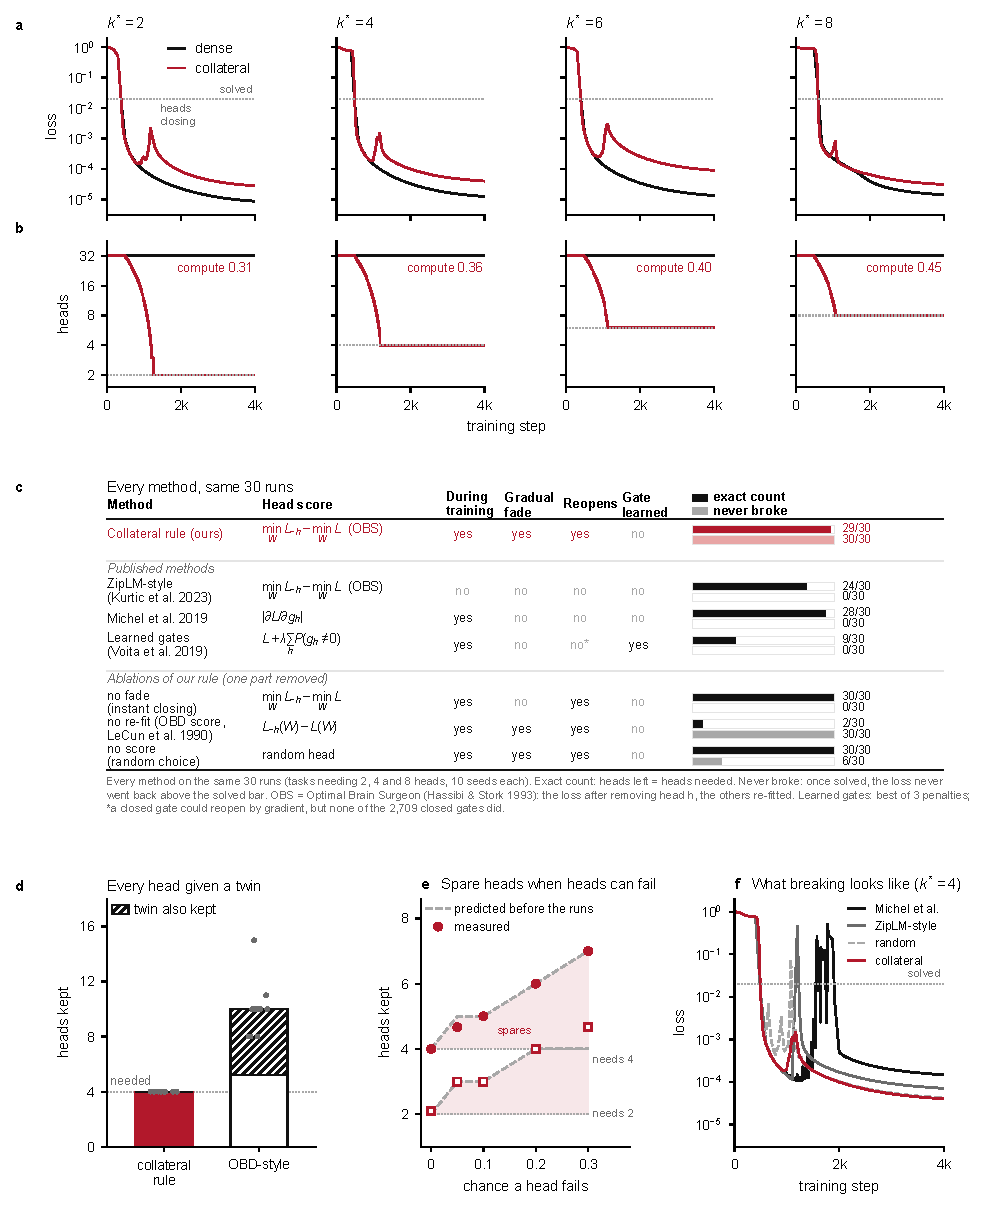
\includegraphics[width=\linewidth]{fig_main.pdf}
\caption{\textbf{Hemodynamic attenuation during training.}
\textbf{a}, Loss of the dense model (black) and with hemodynamic attenuation (red) for $k^\star = 2, 4, 6, 8$
(one seed each); dotted line, the solved bar. The small rise is heads fading out.
\textbf{b}, Number of open heads; dotted line, $k^\star$. ``Compute'' is head-steps used, as a
fraction of the dense model's, including the cost of valuing heads.
\textbf{c}, Every method on the same 30 runs ($k^\star = 2, 4, 8$, 10 seeds each), all run the same way here:
how it scores a head, whether it prunes during training as published, fades heads gradually, and can reopen them,
and how often it kept exactly $k^\star$ heads (dark bar) and never broke the model (light bar). Published methods
above; below, controls that remove one part of our method.
\textbf{d}, Runs that start with every head copied ($k^\star = 4$, 10 runs each; one circle per run): heads
kept, and how many twin pairs kept both copies.
\textbf{e}, Spare heads kept when each head fails with chance $p$ at every step ($k^\star = 4$): one circle
per run (10 runs at $p = 0$, 3 at each other $p$), against the number predicted before the runs (dashed).
\textbf{f}, One run of each method ($k^\star = 4$, seed 0): only hemodynamic attenuation stays below the
solved bar.}
\label{fig:main}
\end{figure}

\paragraph{Only hemodynamic attenuation finds the count and never breaks the model.}
Table~\ref{tab:rules} and Figure~\ref{fig:main}c. Each baseline gets at most one of the two
properties. Ordinary importance never breaks the model but keeps too many heads, because it values
heads that copy each other. Random choice and standard pruning reach the right count but break the
model on the way: they close heads that are still needed. Learned gates rarely get either.

\begin{table}[h]
\centering
\begin{tabular}{lccc}
\toprule
rule & runs & exact count & stays solved \\
\midrule
\textbf{hemodynamic attenuation}            & 50 & \textbf{47/50} & \textbf{50/50} \\
ordinary importance                 & 30 & 2/30  & 30/30 \\
random choice                       & 30 & 30/30 & 6/30 \\
standard pruning \citep{michel}     & 36 & 34/36 & 0/36 \\
learned gates, penalty 0.05         & 9  & 0/9   & 1/9 \\
learned gates, penalty 0.2          & 9  & 0/9   & 1/9 \\
learned gates, penalty 1.0          & 9  & 3/9   & 0/9 \\
\bottomrule
\end{tabular}
\caption{\textbf{Count and stability.} $k^\star \in \{2, 3, 4, 6, 8\}$ for hemodynamic attenuation and
standard pruning, $\{2, 4, 8\}$ for the others; 3 to 10 seeds per size.}
\label{tab:rules}
\end{table}

\paragraph{During training versus all at once after.} Table~\ref{tab:oneshot} applies the same
value and the same price in one go. Cut after the task is solved, it finds the count but breaks
the model in every run: the loss jumps to 8 to 22 times the solved bar before fine-tuning repairs
it, and the run uses more compute. Cut early, before the task is solved, the values are not yet
meaningful and the cut goes too deep (2 heads for a 4-head task, 1 for an 8-head task) with no way
back. Doing it gradually during training, with reopening, avoids both failures.

\begin{table}[h]
\centering
\small
\begin{tabular}{lcccc}
\toprule
how the value is used & exact & stays solved & worst loss$/L_{\text{triv}}$ & compute \\
\midrule
\textbf{during training, gradual (ours)} & \textbf{29/30} & \textbf{30/30} & \textbf{0.009--0.012} & 0.27--0.40 \\
all at once at step 1200 (after solved)  & 13/15 & 0/15 & 0.17--0.45 & 0.35--0.48 \\
all at once at step 2000                 & 13/15 & 0/15 & 0.16--0.45 & 0.54--0.63 \\
all at once at step 400 (before solved)  & 3/15  & 5/15 & never solved at $k^\star \ge 4$ & 0.13--0.17 \\
\bottomrule
\end{tabular}
\caption{\textbf{Same value, same price, different use.} $k^\star \in \{2, 4, 8\}$; 10 seeds per size
for the rule, 5 for each one-shot arm. Worst loss is the highest validation loss after the model is
first solved (median per size; the solved bar is 0.02). Compute is head-steps used as a fraction of the dense model's, not counting the cost of computing the values.}
\label{tab:oneshot}
\end{table}

\paragraph{Duplicate heads are removed.} If every head starts as an exact copy of another
(Figure~\ref{fig:main}d), hemodynamic attenuation keeps 4 heads and never both members of a pair
(10 of 10 runs), because a copy is fully covered by its twin. Ordinary importance keeps 8 to 15
heads, with 4 to 7 pairs kept twice. With near-copies (twin = copy plus noise of 10\% of the
weights' spread) hemodynamic attenuation still kept exactly 4 heads in 5 of 5 runs, while ordinary
importance kept 5 to 10. In 2 of the 5 runs both members of one pair were among the four; since
four heads solved the task, those twins had drifted apart into different jobs. With larger noise (50\%) the picture was the same: hemodynamic attenuation kept exactly 4 heads in 5 of 5 runs, ordinary importance 5 to 9.

\paragraph{Cost.} The rule's final loss is 2 to 7 times that of the dense model (Figure~\ref{fig:main}a),
always far below the solved bar, using 0.31 to 0.45 of the dense model's head-steps
(Figure~\ref{fig:main}b).

\subsection{Backup heads when heads can fail}
\label{sec:backup}

If each head fails at random (valve forced to 0) with chance $p$ at every step, a head is worth
keeping only if it is likely to be needed. With $B$ heads open, $R$ needed, and each head working
with chance $1 - p$, a head contributes when it works and fewer than $R$ of the other $B - 1$ do:
\begin{equation}
v(B) = \frac{1 - p}{R}\; \Pr\big[\,\text{Binomial}(B - 1,\, 1 - p) < R\,\big].
\end{equation}
The rule keeps heads while $v(B)$ is above the price, so the predicted count is the largest $B$
with $v(B) \ge$ price. We wrote these predictions down before running the experiments
(Table~\ref{tab:backup}, Figure~\ref{fig:main}e): 21 of 24 runs matched exactly, the other three
were off by one head. One caveat: the rule estimates the same marginal value that the formula
computes in expectation, so the match shows that the rule behaves as designed under failures; it
does not show that every trained network would keep this many backups.

\begin{table}[h]
\centering
\begin{tabular}{ccccccccc}
\toprule
& \multicolumn{4}{c}{$R = 2$} & \multicolumn{4}{c}{$R = 4$} \\
\cmidrule(lr){2-5}\cmidrule(lr){6-9}
failure chance $p$ & 0.05 & 0.1 & 0.2 & 0.3 & 0.05 & 0.1 & 0.2 & 0.3 \\
\midrule
predicted & 3 & 3 & 4 & 4 & 5 & 5 & 6 & 7 \\
measured (3 seeds) & 3, 3, 3 & 3, 3, 3 & 4, 4, 4 & 5, 4, 5 & 5, 5, 4 & 5, 5, 5 & 6, 6, 6 & 7, 7, 7 \\
\bottomrule
\end{tabular}
\caption{\textbf{Backup heads}, predicted before the runs and measured.}
\label{tab:backup}
\end{table}

\subsection{A second circuit: two-layer induction}

To check the rule beyond one layer, we trained a 2-layer attention-only model (8 + 8 heads) on
induction: a random sequence of 8 tokens appears, then after a gap it repeats, and the model must
predict each next token of the repeat. The known minimal circuit is one previous-token head in
layer 1 and one induction head in layer 2 \citep{olsson}; a dense 1 + 1 model solves the task. With
a loss-based value, the rule kept 2 + 1 heads in 10 of 10 runs, stayed solved in 10 of 10, and the
kept heads had the expected roles. It did not reach the minimal 1 + 1, although a 1 + 1 model trained from scratch solves the task. Forcing trial closures reached 1 + 1 in 8 of 20 runs, but 3 of the 20 did not end solved,
so on this task the exact count and stability trade off.

\section{Related work}

\emph{Pruning scores.} Optimal Brain Damage and Optimal Brain Surgeon \citep{obd,obs} value a weight
by the loss change after the remaining weights compensate. ZipLM \citep{ziplm} applies this to whole
heads and MLP neurons of a trained language model toward a chosen speed-up, and \citet{kwon} pick
heads for a compute budget and rescale the rest by least squares. Our value is the same idea; we
differ in using it from the start of training, with a price and no target, gradually and with
reopening, and in testing whether it recovers a known minimal count while staying solved.
\emph{Head pruning.} \citet{michel} showed many heads can be removed after training; \citet{voita}
learned head gates with an L0 penalty \citep{louizos}. Both are our baselines.
\emph{Circuits and redundancy.} Circuit discovery is usually post hoc \citep{acdc}. Trained models
contain backup heads that take over when others are removed \citep{ioi,hydra}; we predict how many
backups our rule keeps under random failure.

\section{Limitations}

The tasks are small and the model has one layer (two for induction) with no MLP; the point is that
the minimal count is known, which is not true of real language models. The value is computed with
a linear re-fit of the output weights, exact for this one-layer model and only an approximation in
deeper ones; on induction the rule kept one head more than needed. The final loss is 2 to 7 times
the dense model's. The blood-flow analogy motivates the rule but is not evidence for it.

\begin{thebibliography}{99}\setlength{\itemsep}{2pt}\small
\bibitem[Conmy et al.(2023)]{acdc} A.~Conmy, A.~Mavor-Parker, A.~Lynch, S.~Heimersheim, A.~Garriga-Alonso.
  Towards automated circuit discovery for mechanistic interpretability. \emph{NeurIPS}, 2023.
\bibitem[Hassibi and Stork(1993)]{obs} B.~Hassibi, D.~Stork. Second order derivatives for network
  pruning: Optimal Brain Surgeon. \emph{NeurIPS}, 1993.
\bibitem[Kurtic et al.(2023)]{ziplm} E.~Kurtic, E.~Frantar, D.~Alistarh. ZipLM: Inference-aware
  structured pruning of language models. \emph{NeurIPS}, 2023.
\bibitem[Kwon et al.(2022)]{kwon} W.~Kwon, S.~Kim, M.~Mahoney, J.~Hassoun, K.~Keutzer, A.~Gholami.
  A fast post-training pruning framework for transformers. \emph{NeurIPS}, 2022.
\bibitem[LeCun et al.(1989)]{obd} Y.~LeCun, J.~Denker, S.~Solla. Optimal brain damage. \emph{NeurIPS}, 1989.
\bibitem[Louizos et al.(2018)]{louizos} C.~Louizos, M.~Welling, D.~Kingma. Learning sparse neural
  networks through $L_0$ regularization. \emph{ICLR}, 2018.
\bibitem[McGrath et al.(2023)]{hydra} T.~McGrath, M.~Rahtz, J.~Kram\'ar, V.~Mikulik, S.~Legg.
  The Hydra effect: emergent self-repair in language model computations. arXiv:2307.15771, 2023.
\bibitem[Michel et al.(2019)]{michel} P.~Michel, O.~Levy, G.~Neubig. Are sixteen heads really better
  than one? \emph{NeurIPS}, 2019.
\bibitem[Olsson et al.(2022)]{olsson} C.~Olsson et al. In-context learning and induction heads.
  \emph{Transformer Circuits Thread}, 2022.
\bibitem[Voita et al.(2019)]{voita} E.~Voita, D.~Talbot, F.~Moiseev, R.~Sennrich, I.~Titov. Analyzing
  multi-head self-attention: specialized heads do the heavy lifting, the rest can be pruned. \emph{ACL}, 2019.
\bibitem[Wang et al.(2023)]{ioi} K.~Wang, A.~Variengien, A.~Conmy, B.~Shlegeris, J.~Steinhardt.
  Interpretability in the wild: a circuit for indirect object identification in GPT-2 small. \emph{ICLR}, 2023.
\end{thebibliography}

\end{document}
